\documentclass[landscape,a0paper,fontscale=0.292]{baposter}

\usepackage[vlined]{algorithm2e}
\usepackage{times}
\usepackage{calc}
\usepackage{url}
\usepackage{graphicx}
\usepackage{amsmath}
\usepackage{amssymb}
\usepackage{relsize}
\usepackage{multirow}
\usepackage{booktabs}
\usepackage{makecell}
\usepackage{threeparttable}
\usepackage{subfig}
\usepackage{graphbox}

\usepackage{multicol}
\usepackage[T1]{fontenc}
\usepackage{ae}
\usepackage{enumitem}

\usepackage{colortbl}
\usepackage{xcolor}

\definecolor{darkcyan}{HTML}{90ee90}
% \definecolor{darkcyan}{HTML}{82df83}
\definecolor{ctitle}{HTML}{00a900}

\usepackage[pagebackref=true,breaklinks=true,colorlinks=true,bookmarks=false,linkcolor={red!50!black},urlcolor={magenta},citecolor={green!50!black}]{hyperref} 

\setlist[itemize]{leftmargin=*,nosep}
    \setlength{\columnsep}{0.7em}
    \setlength{\columnseprule}{0mm}

\setlist[enumerate]{leftmargin=2.5em,nosep}
    \setlength{\columnsep}{1.0em}
    \setlength{\columnseprule}{0mm}

% %%%%%%%%%%%%%%%%%%%%%%%%%%%%%%%%%%%%%%%%%%%%%%%%%%%%%%%%%%%%%%%%%%%%%%%%%%%%%%%%
% % Save space in lists. Use this after the opening of the list
% %%%%%%%%%%%%%%%%%%%%%%%%%%%%%%%%%%%%%%%%%%%%%%%%%%%%%%%%%%%%%%%%%%%%%%%%%%%%%%%%
% \newcommand{\compresslist}{%
% \setlength{\itemsep}{0pt}%
% \setlength{\itemsep}{0pt}%
% \setlength{\parskip}{0pt}%
% \setlength{\parsep}{0pt}%
% }
\renewcommand{\rmdefault}{ptm} % Arial
\renewcommand{\sfdefault}{ptm} % Arial

\newcommand{\lout}{\hat{I}}
\newcommand{\lin}{L_i}
\newcommand{\din}{\boldsymbol{w}_i}
\newcommand{\dout}{\boldsymbol{w}_o}
\newcommand{\normal}{\boldsymbol{n}}
\newcommand{\brdf}{f_r}
\newcommand{\vmlp}{f_v}
\newcommand{\point}{\boldsymbol{x}}
%%%%%%%%%%%%%%%%%%%%%%%%%%%%%%%%%%%%%%%%%%%%%%%%%%%%%%%%%%%%%%%%%%%%%%%%%%%%%
%% Begin of Document
%%%%%%%%%%%%%%%%%%%%%%%%%%%%%%%%%%%%%%%%%%%%%%%%%%%%%%%%%%%%%%%%%%%%%%%%%%%%%
\begin{document}
%%%%%%%%%%%%%%%%%%%%%%%%%%%%%%%%%%%%%%%%%%%%%%%%%%%%%%%%%%%%%%%%%%%%%%%%%%%%%
%% Here starts the poster
%%---------------------------------------------------------------------------
%% Format it to your taste with the options
%%%%%%%%%%%%%%%%%%%%%%%%%%%%%%%%%%%%%%%%%%%%%%%%%%%%%%%%%%%%%%%%%%%%%%%%%%%%%
\begin{poster}{
    % Show grid to help with alignment
    grid=false,
    columns=6,
    % Column spacing
    colspacing=0.7em,
    % Color style
    headerColorOne=darkcyan,
    borderColor=darkcyan,
    % Format of textbox
    textborder=faded,
    % Format of text header
    headerborder=open,
    headershape=roundedright,
    headershade=plain,
    background=none,
    bgColorOne=cyan!10!white,
    headerheight=0.13\textheight
}
% Eye Catcher
{
    % \begin{tabular}{c}
    %     \raisebox{-1.0\height}{
\includegraphics[height=0.0445\linewidth]{logo/shanghaitech-emblem.pdf}}
    %     \makebox[0.005\textwidth]{} 
    %     \raisebox{-1.0\height}{
\includegraphics[height=0.0445\linewidth]{logo/HKU}}\\
    %     \raisebox{-0.4\height}{
\includegraphics[height=0.0445\linewidth]{logo/sjtulogored.pdf}}
    %     \makebox[0.005\textwidth]{} 
    %     \raisebox{-0.4\height}{\includegraphics[height=0.0445\linewidth]{logo/MIT-IBM}}
    % \end{tabular}
    \raisebox{0.07\height}{
\includegraphics[height=0.0445\linewidth]{logo/shanghaitech-emblem.pdf}}
    \makebox[0.005\textwidth]{} 
    \raisebox{0.07\height}{
\includegraphics[height=0.0445\linewidth]{logo/XiaohongshuLOGO.svg.png}}
    \makebox[0.005\textwidth]{} 
    \raisebox{0.07\height}{
\includegraphics[height=0.0445\linewidth]{logo/HKU}}
    \makebox[0.005\textwidth]{}
    \raisebox{0.07\height}{
\includegraphics[height=0.0445\linewidth]{logo/sjtulogored.pdf}}
}
% Title
{
    \\[0.3em]\sc\huge\bf \textcolor{ctitle}{GeoFormer}: Learning Point Cloud Completion with Tri-Plane Integrated Transformer
}
% Authors
{
    \vspace{0.3em} Jinpeng Yu$^{1,2}$ \enspace Binbin Huang$^3$ \enspace Yuxuan Zhang$^4$ \enspace Huaxia Li$^2$ \enspace Xu Tang$^2$ \enspace Shenghua Gao$^3$ \\[0.2em]
    {$^1$ShanghaiTech University \enspace$^2$Xiaohongshu Inc. \\[0.1em] $^3$The University of Hong Kong \enspace$^4$Shanghai Jiao Tong University}
}
% University logo
{
    \begin{tabular}{c}
        \raisebox{-1.0\height}{
\includegraphics[align=c,width=0.1\linewidth]{logo/mm_logo_nobg.png}}\\
        \raisebox{-0.7\height}{
        
\includegraphics[align=c,width=0.095\linewidth]{logo/link.pdf}\hspace{0.002\linewidth}
        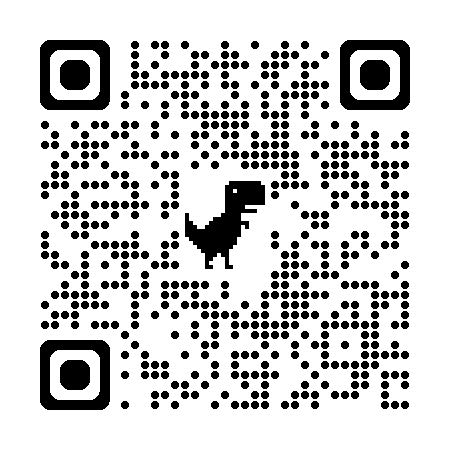
\includegraphics[align=c,height=0.035\linewidth]{logo/qrcode_github.com.png}}
    \end{tabular}
}

%%%%%%%%%%%%%%%%%%%%%%%%%%%%%%%%%%%%%%%%%%%%%%%%%%%%%%%%%%%%%%%%%%%%%%%%%%%%%%
%%% Now define the boxes that make up the poster
%%%---------------------------------------------------------------------------
%%% Each box has a name and can be placed absolutely or relatively.
%%% The only inconvenience is that you can only specify a relative position 
%%% towards an already declared box. So if you have a box attached to the 
%%% bottom, one to the top and a third one which should be inbetween, you 
%%% have to specify the top and bottom boxes before you specify the middle 
%%% box.
%%%%%%%%%%%%%%%%%%%%%%%%%%%%%%%%%%%%%%%%%%%%%%%%%%%%%%%%%%%%%%%%%%%%%%%%%%%%%%

%%%%%%%%%%%%%%%%%%%%%%%%%%%%%%%%%%%%%%%%%%%%%%%%%%%%%%%%%%%%%%%%%%%%%%%%%%%%%%
\headerbox{\bf\color{ctitle} Problem and Contribution}{name=contribution,column=0,row=0,span=2}{
    \textbf{\color{ctitle}Idea:}
    GeoFormer simultaneously enhances the global geometric structure and local details of the point cloud by imposing the multi-view consistent canonical coordinate maps (CCMs). \\
    \vspace{-2.0em}
    \begin{center}
        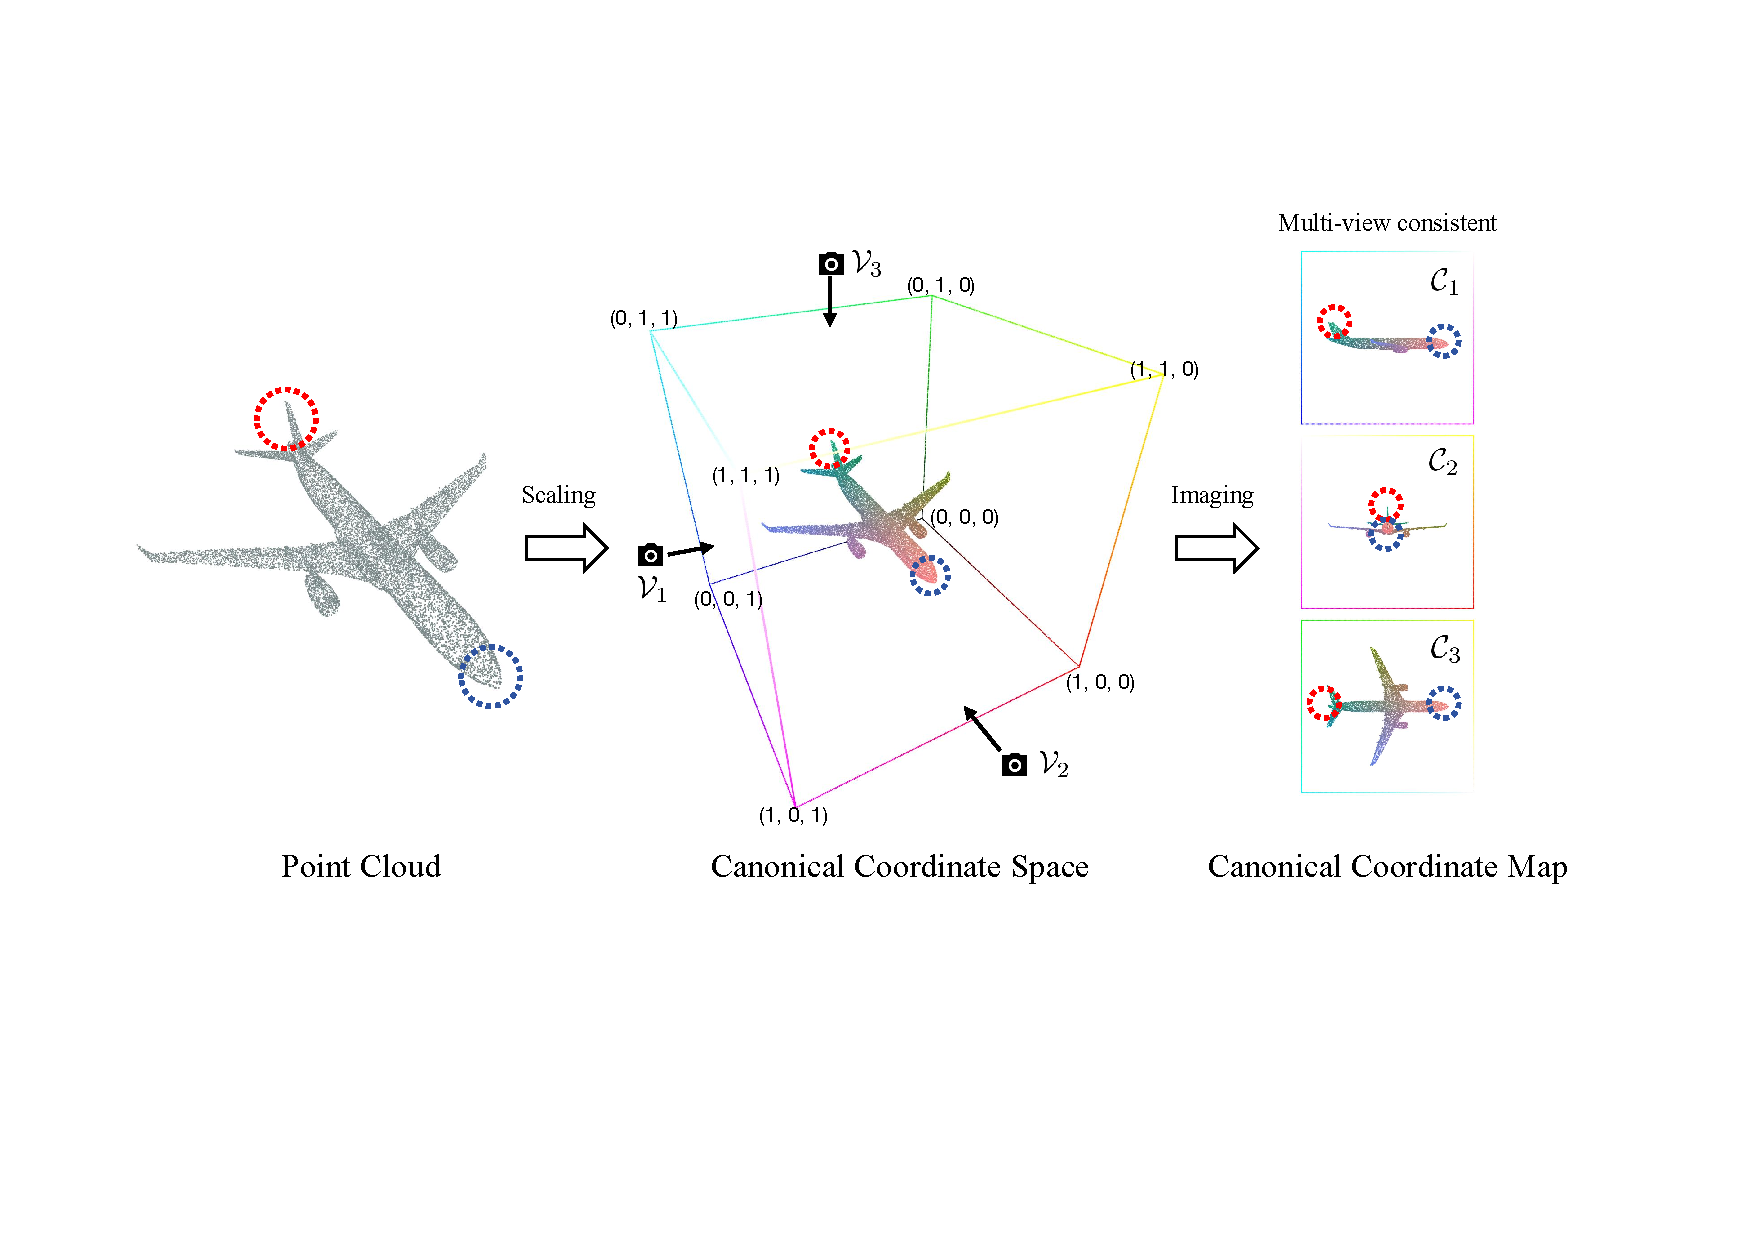
\includegraphics[width=0.8\textwidth]{images/model-teaser.pdf}
    \end{center}
    \vspace{-1.5em}
    \textbf{\color{ctitle}Contributions:}
    \begin{itemize}
        \item We introduce multi-view consistent CCMs into point cloud completion, enhancing global features by aligning 3D and 2D features.
        \item An efficient multi-scale geometry-aware upsampler that accurately reconstructs missing parts by incorporating partial geometric features.
        \item Our method achieves state-of-the-art results. 
    \end{itemize}
    \vspace{-0.6em}
}

\headerbox{\bf\color{ctitle} Method}{name=method,column=0,below=contribution,span=2}{
    \textbf{\color{ctitle}Overview:}
    GeoFormer mainly consists of one point generator module and two identical upsampler modules. The generator module aims to produce sparse yet structurally complete point clouds, and the upsampler module aims to generate complete and dense results from coarse to fine. \\
    \vspace{-1.8em}
    \begin{center}
        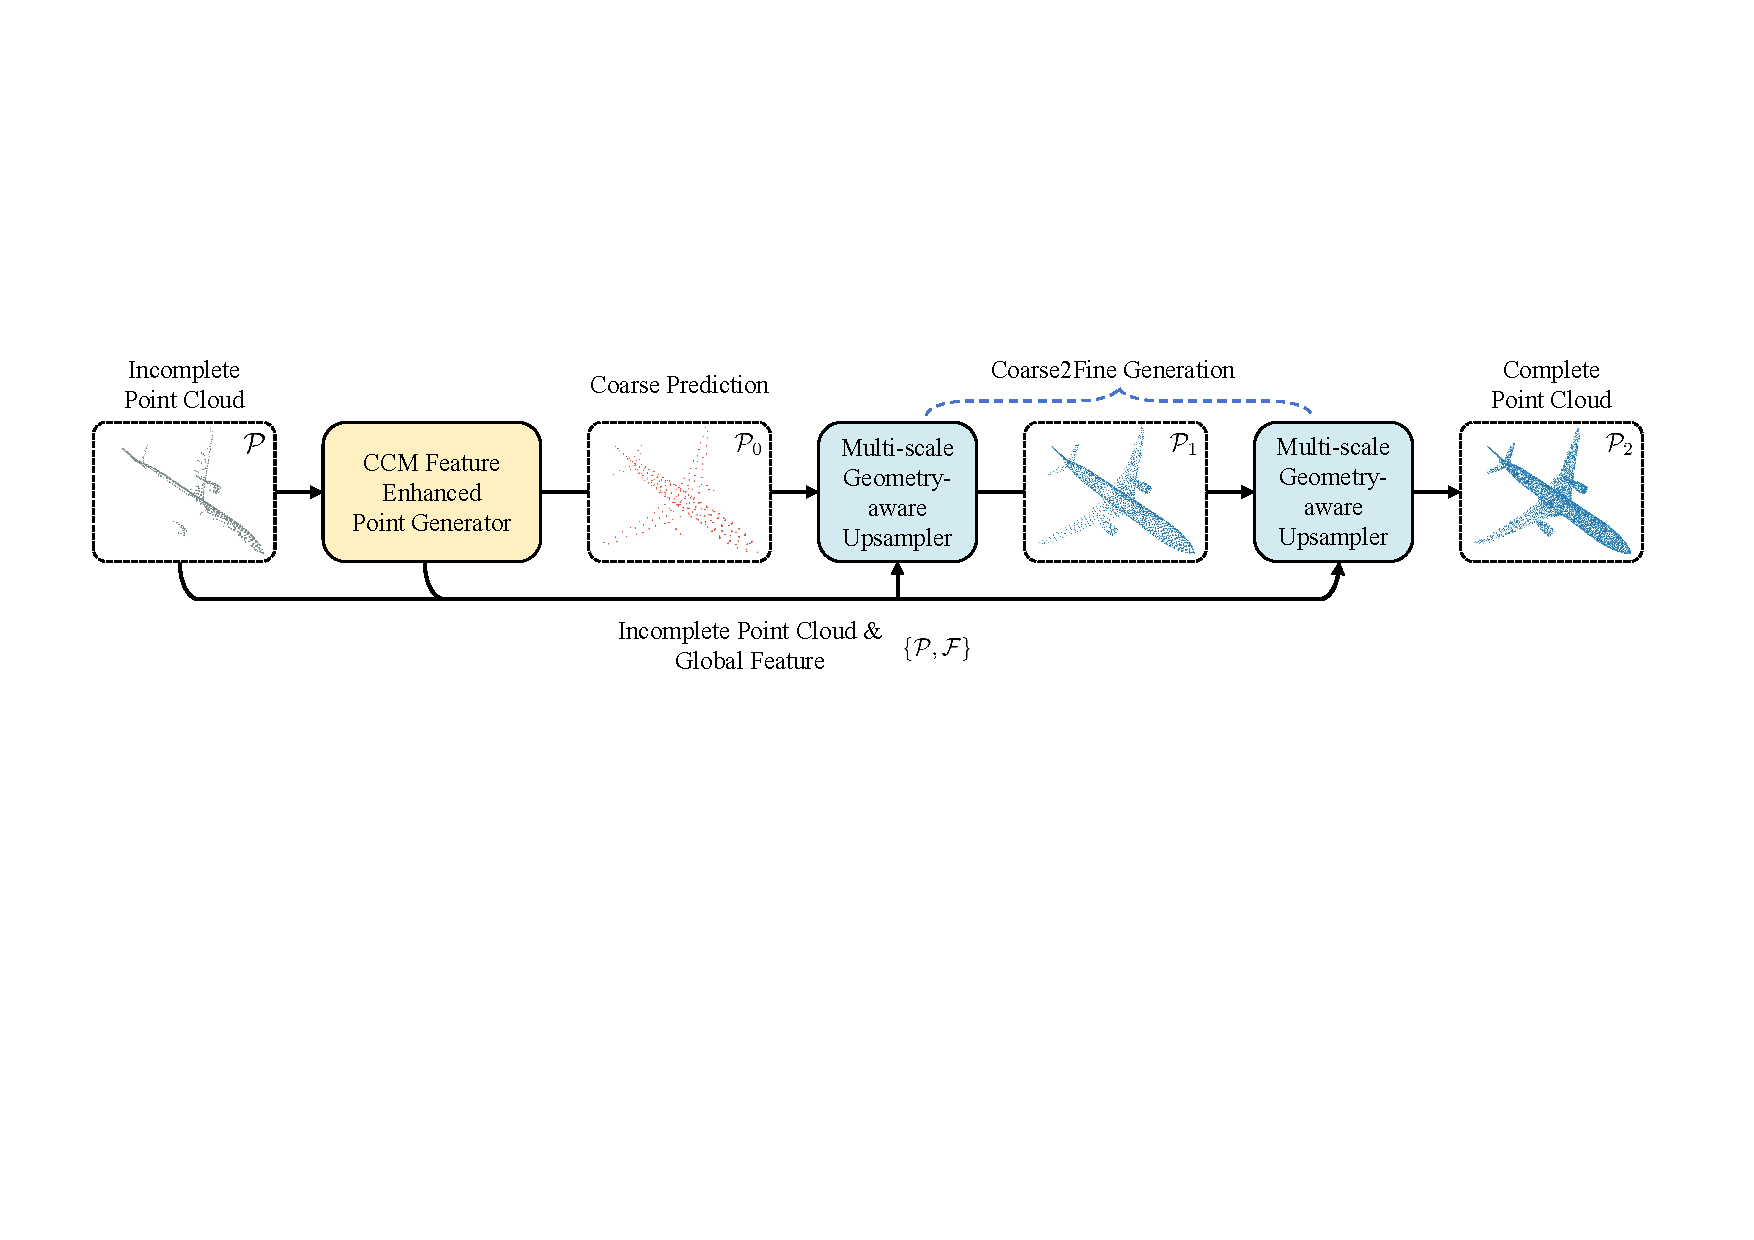
\includegraphics[width=0.95\textwidth]{images/model-pipeline.pdf}
    \end{center}
    \vspace{-1.2em}
    \textbf{\color{ctitle}CCM Feature Enhanced Point Generator:} \\
    We first extract CCMs according to the views $\mathcal{V}$, and then align the 3D and 2D features through attention mechanism to obtain the global feature $\mathcal{F}$. Finally, we use the decoder to predict the coarse point cloud $\mathcal{P}_0$. \\
    \begin{minipage}[c]{0.32\textwidth}
        \begin{center}
            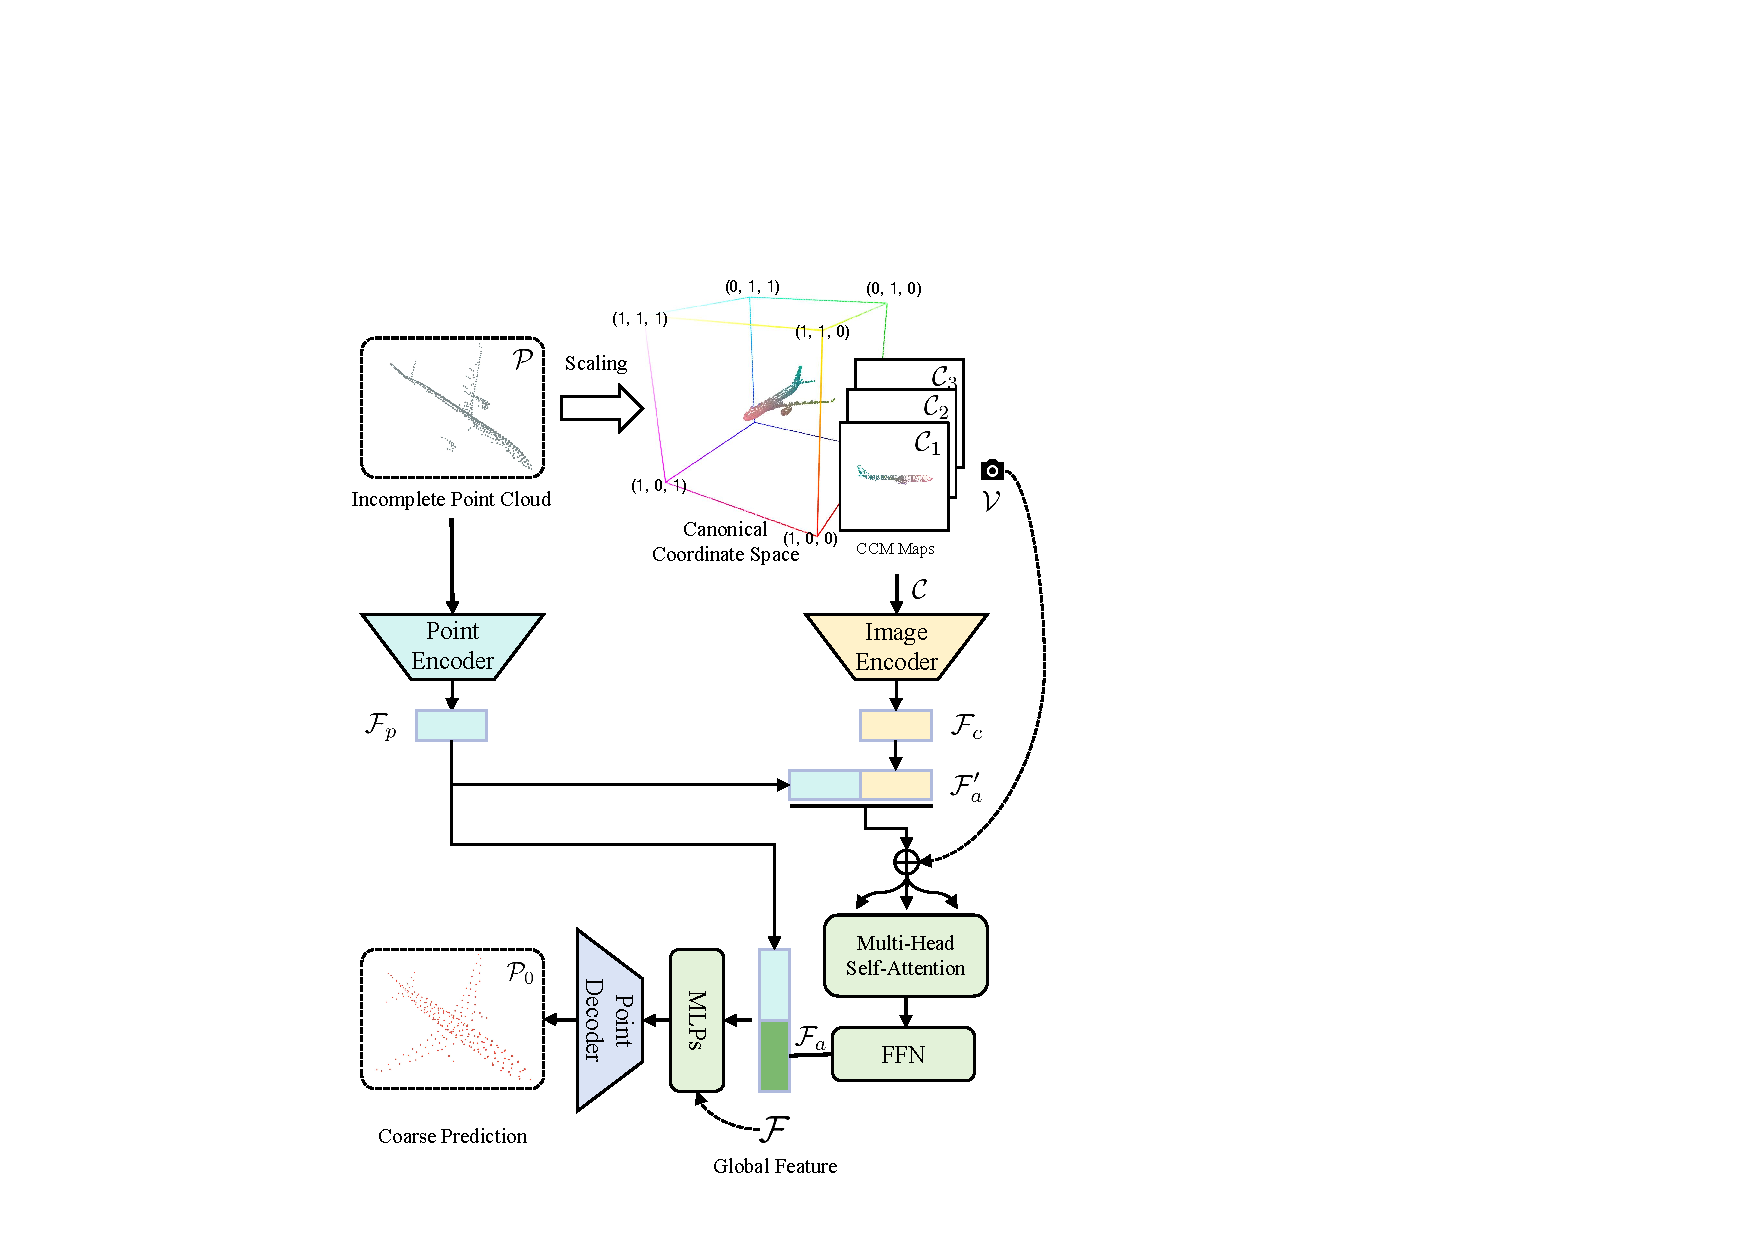
\includegraphics[width=\textwidth]{images/model-generator.pdf}
        \end{center}
    \end{minipage}
    \begin{minipage}[c]{0.68\textwidth}
        \begin{center}
            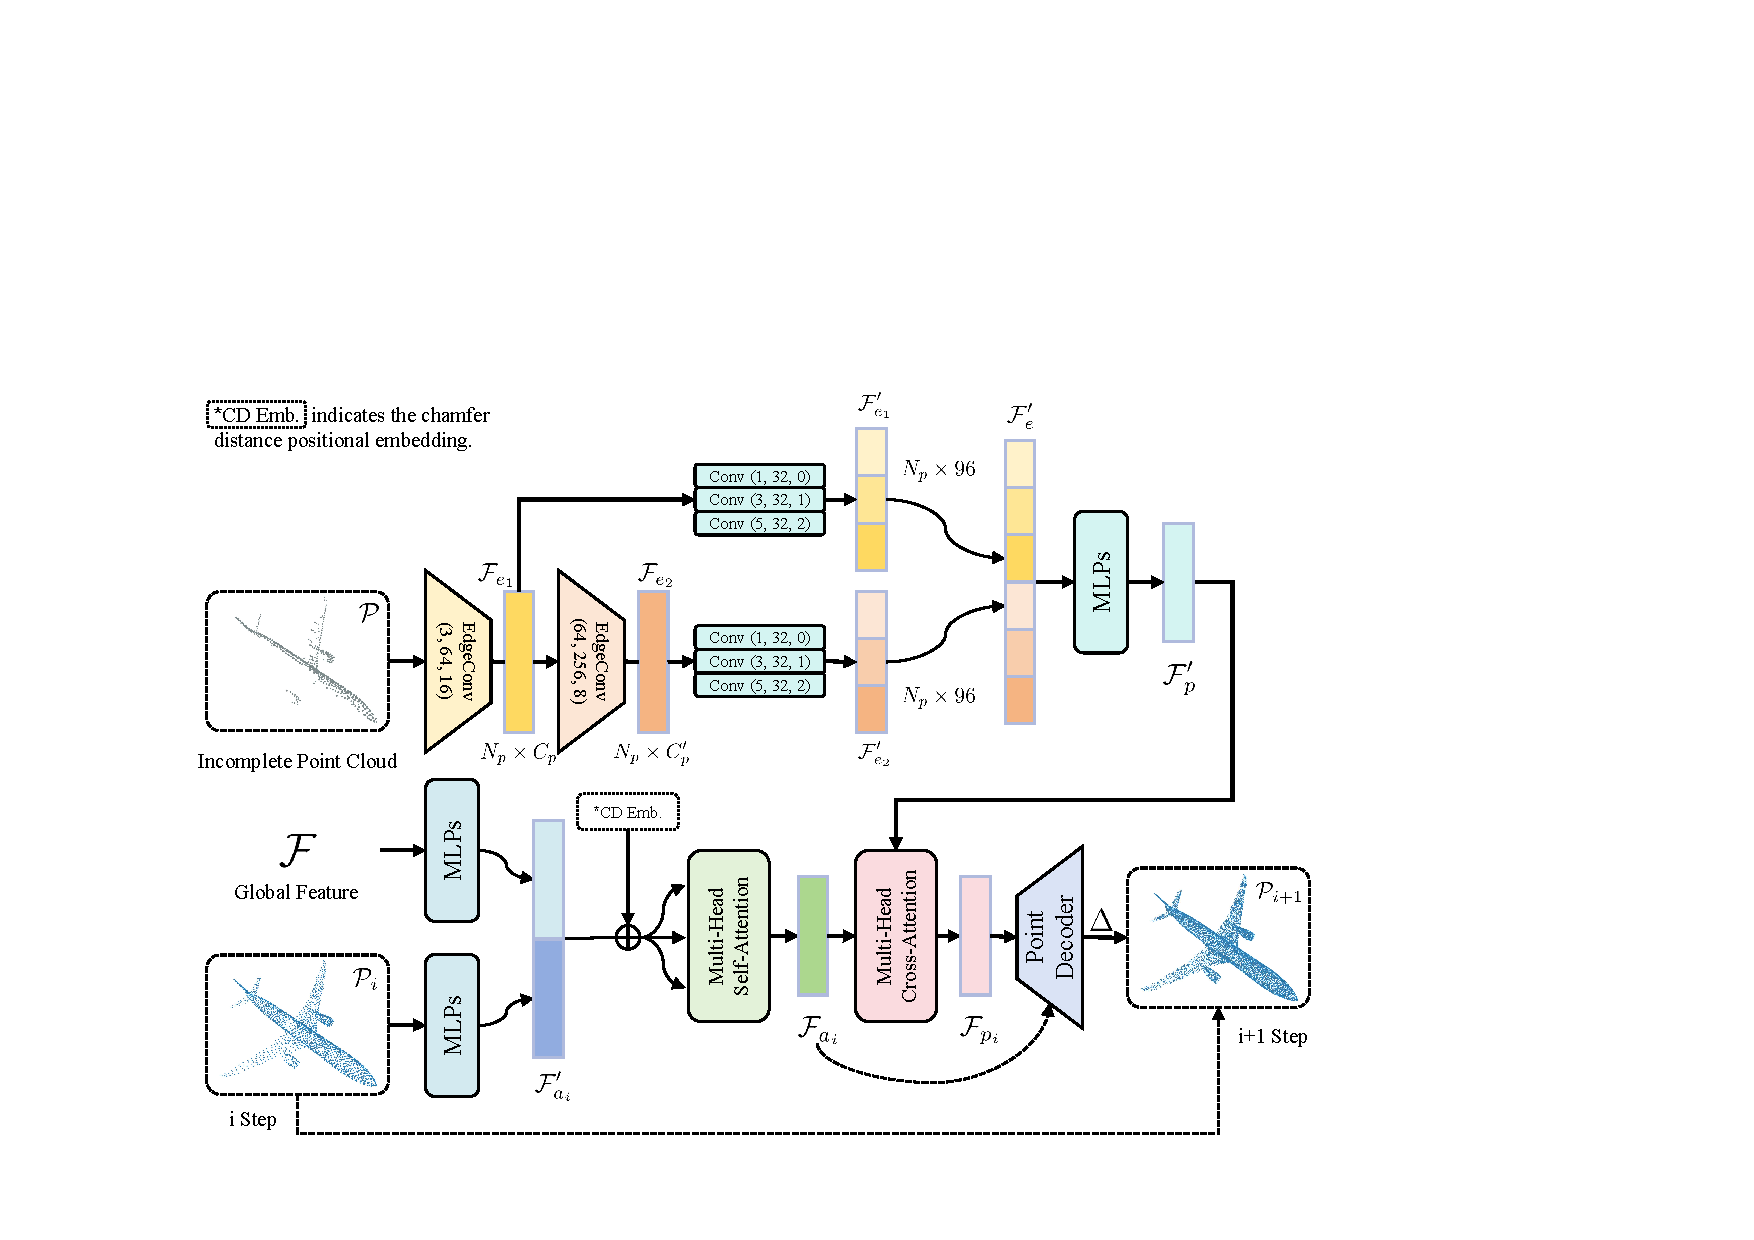
\includegraphics[width=0.95\textwidth]{images/model-upsampler.pdf}
        \end{center}
    \end{minipage}
    \textbf{\color{ctitle}Multi-scale Geometry-aware Upsampler:}  \\
    We first obtain the multi-scale local point features $\mathcal{F}_p^{\prime}$, and then fuse it with the global feature $\mathcal{F}$ and previous $\mathcal{P}_i$ to predict the fine point cloud $\mathcal{P}_{i+1}$. \\
}
%
\headerbox{\bf\color{ctitle} Experiments \& Results}{name=results,column=2,row=0,span=4}{
    \begin{minipage}[t]{0.49\textwidth}
        %%%%%%%%%%%%%%%%%%%%%%%% PCN  %%%%%%%%%%%%%%%%%%%%%%%%%%%%%
        \textbf{\color{ctitle}Comparison on PCN Benchmark:}
        %%%%%%%%%%%%%%%%%%%%%%%% table  %%%%%%%%%%%%%%%%%%%%%%%%%%%%%
        % \vspace{0.2em}
        \vspace{-0.6em}
        \begin{center}
            % Quantitative results on PCN benchmark \\
            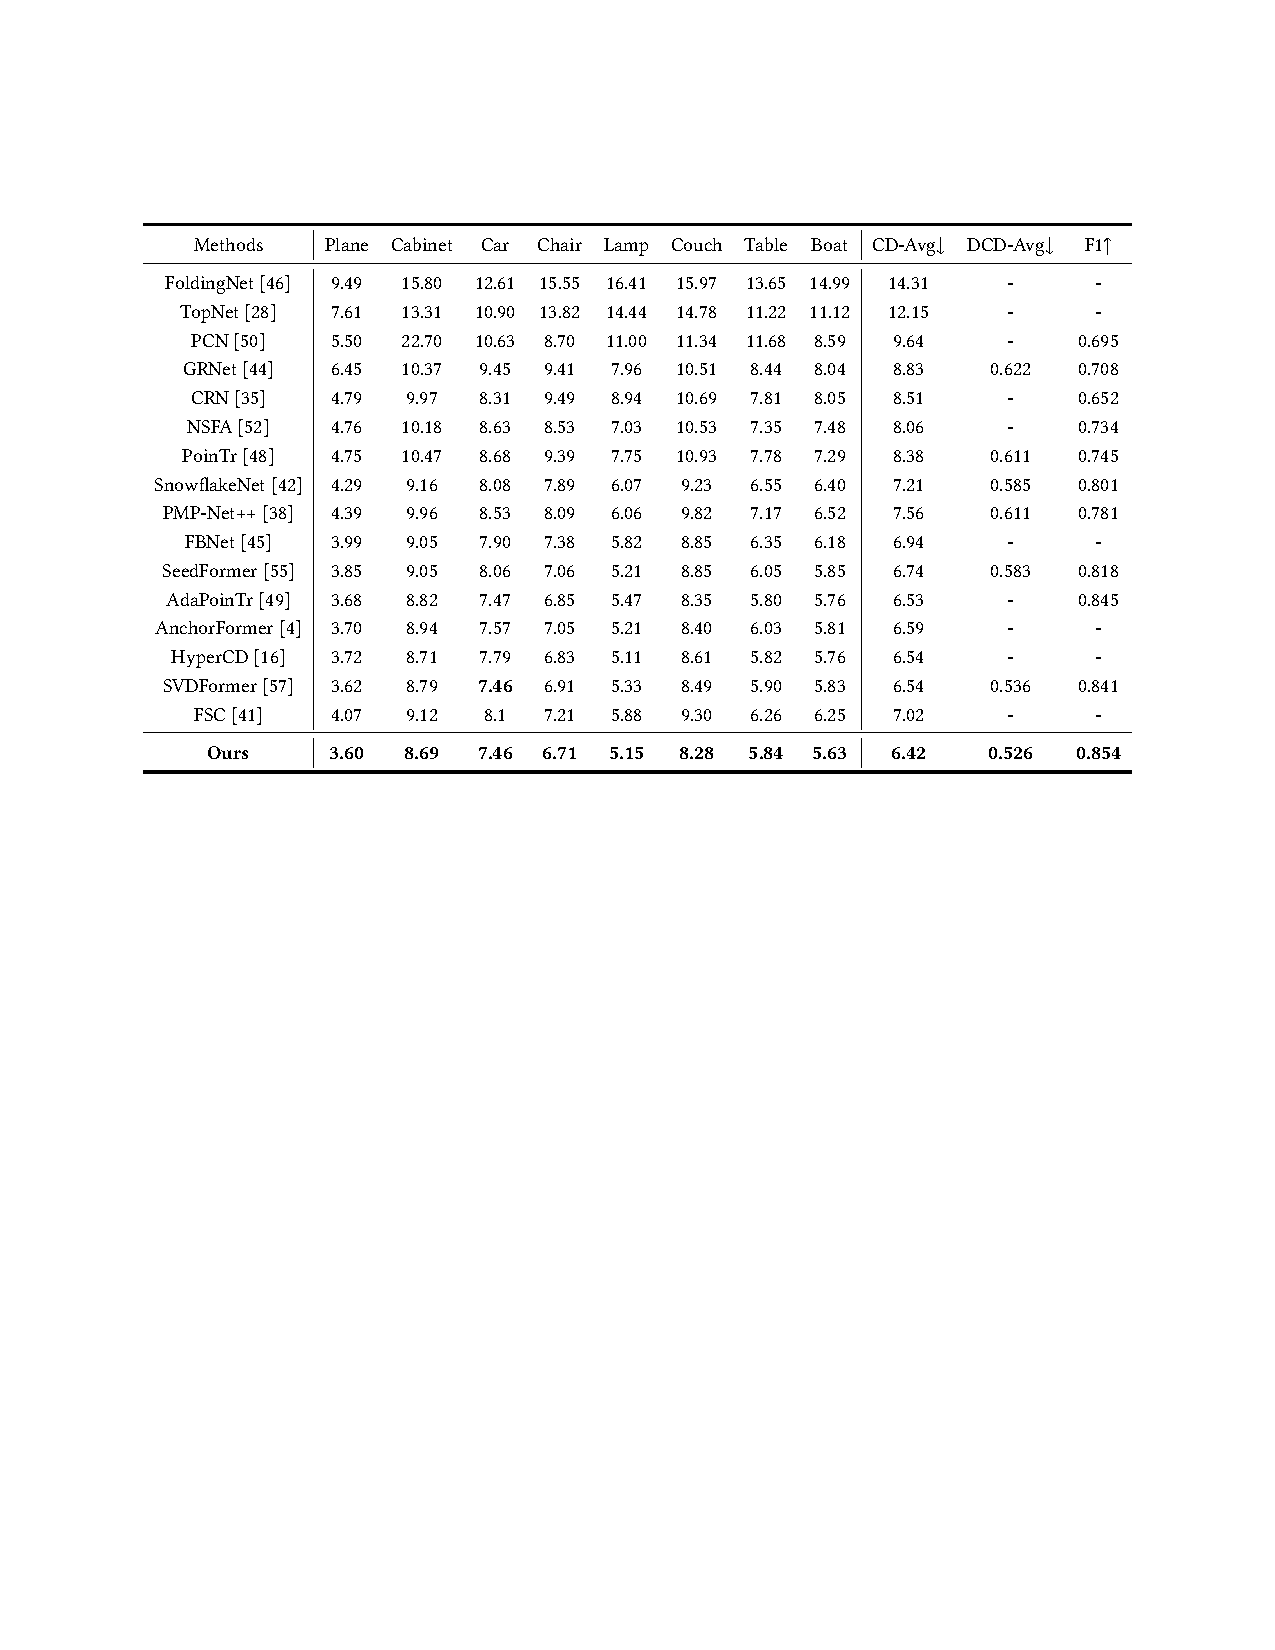
\includegraphics[width=\textwidth]{images/table-PCN.pdf}
        \end{center}
        \vspace{-1.5em}
        %%%%%%%%%%%%%%%%%%%%%%%% figure  %%%%%%%%%%%%%%%%%%%%%%%%%%%%%
        \begin{center}
            % Qualitative results on PCN benchmark \\
            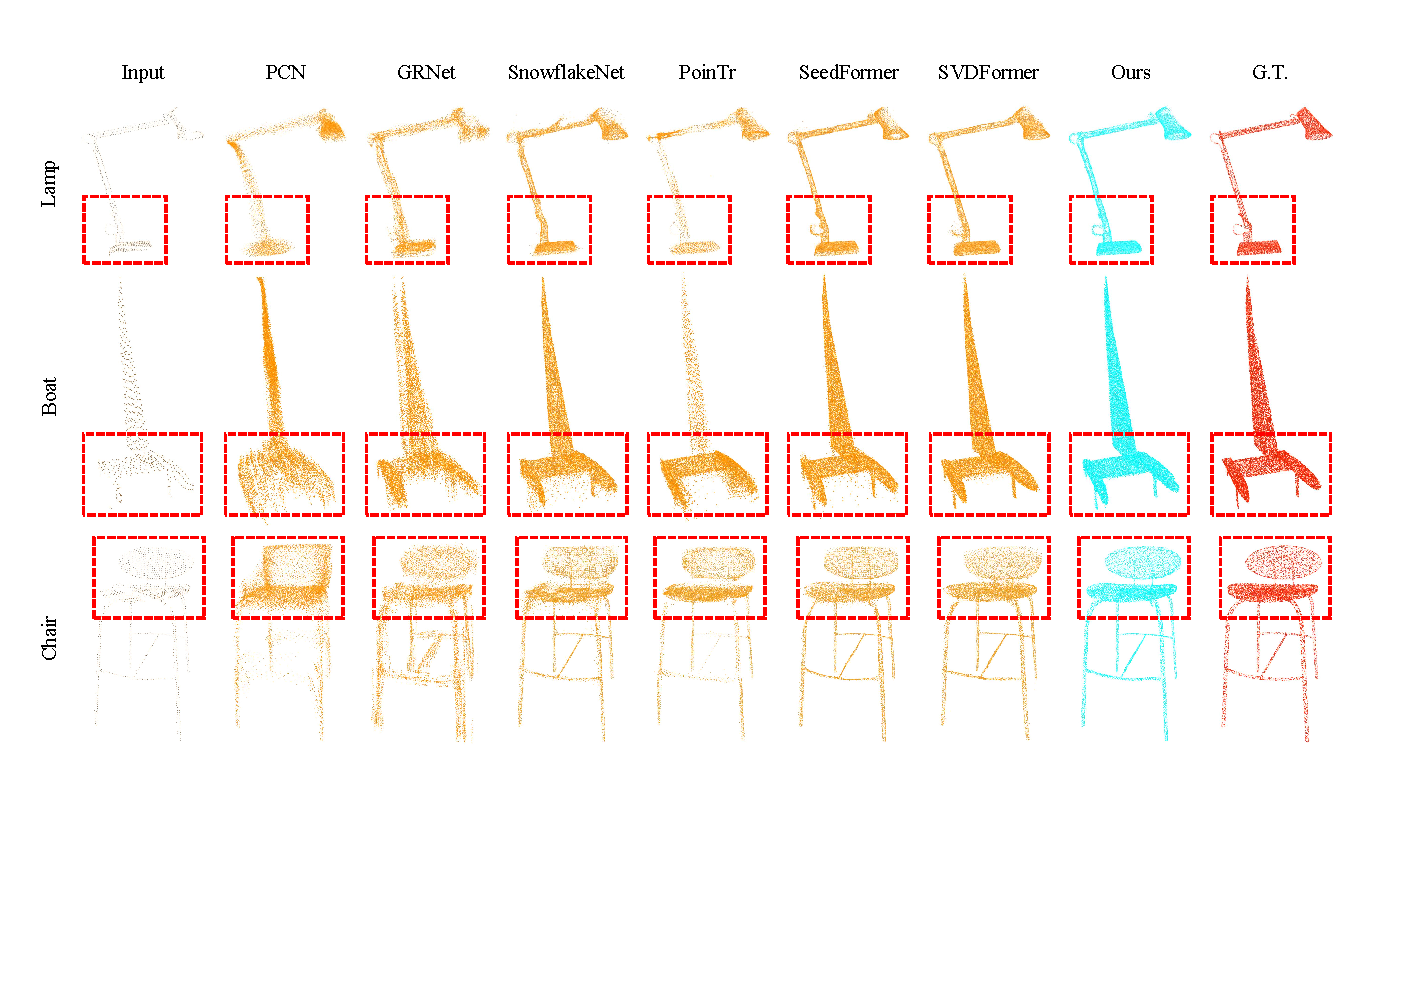
\includegraphics[width=\textwidth]{images/result-pcn.pdf}
        \end{center}
        %%%%%%%%%%%%%%%%%%%%%%%% KITTI  %%%%%%%%%%%%%%%%%%%%%%%%%%%%%
        \vspace{-1.0em}
        \textbf{\color{ctitle}Comparison on KITTI Benchmark:}
        %%%%%%%%%%%%%%%%%%%%%%%% table  %%%%%%%%%%%%%%%%%%%%%%%%%%%%%
        \vspace{-0.5em}
        \begin{center}
            % Quantitative results on KITTI benchmark \\
            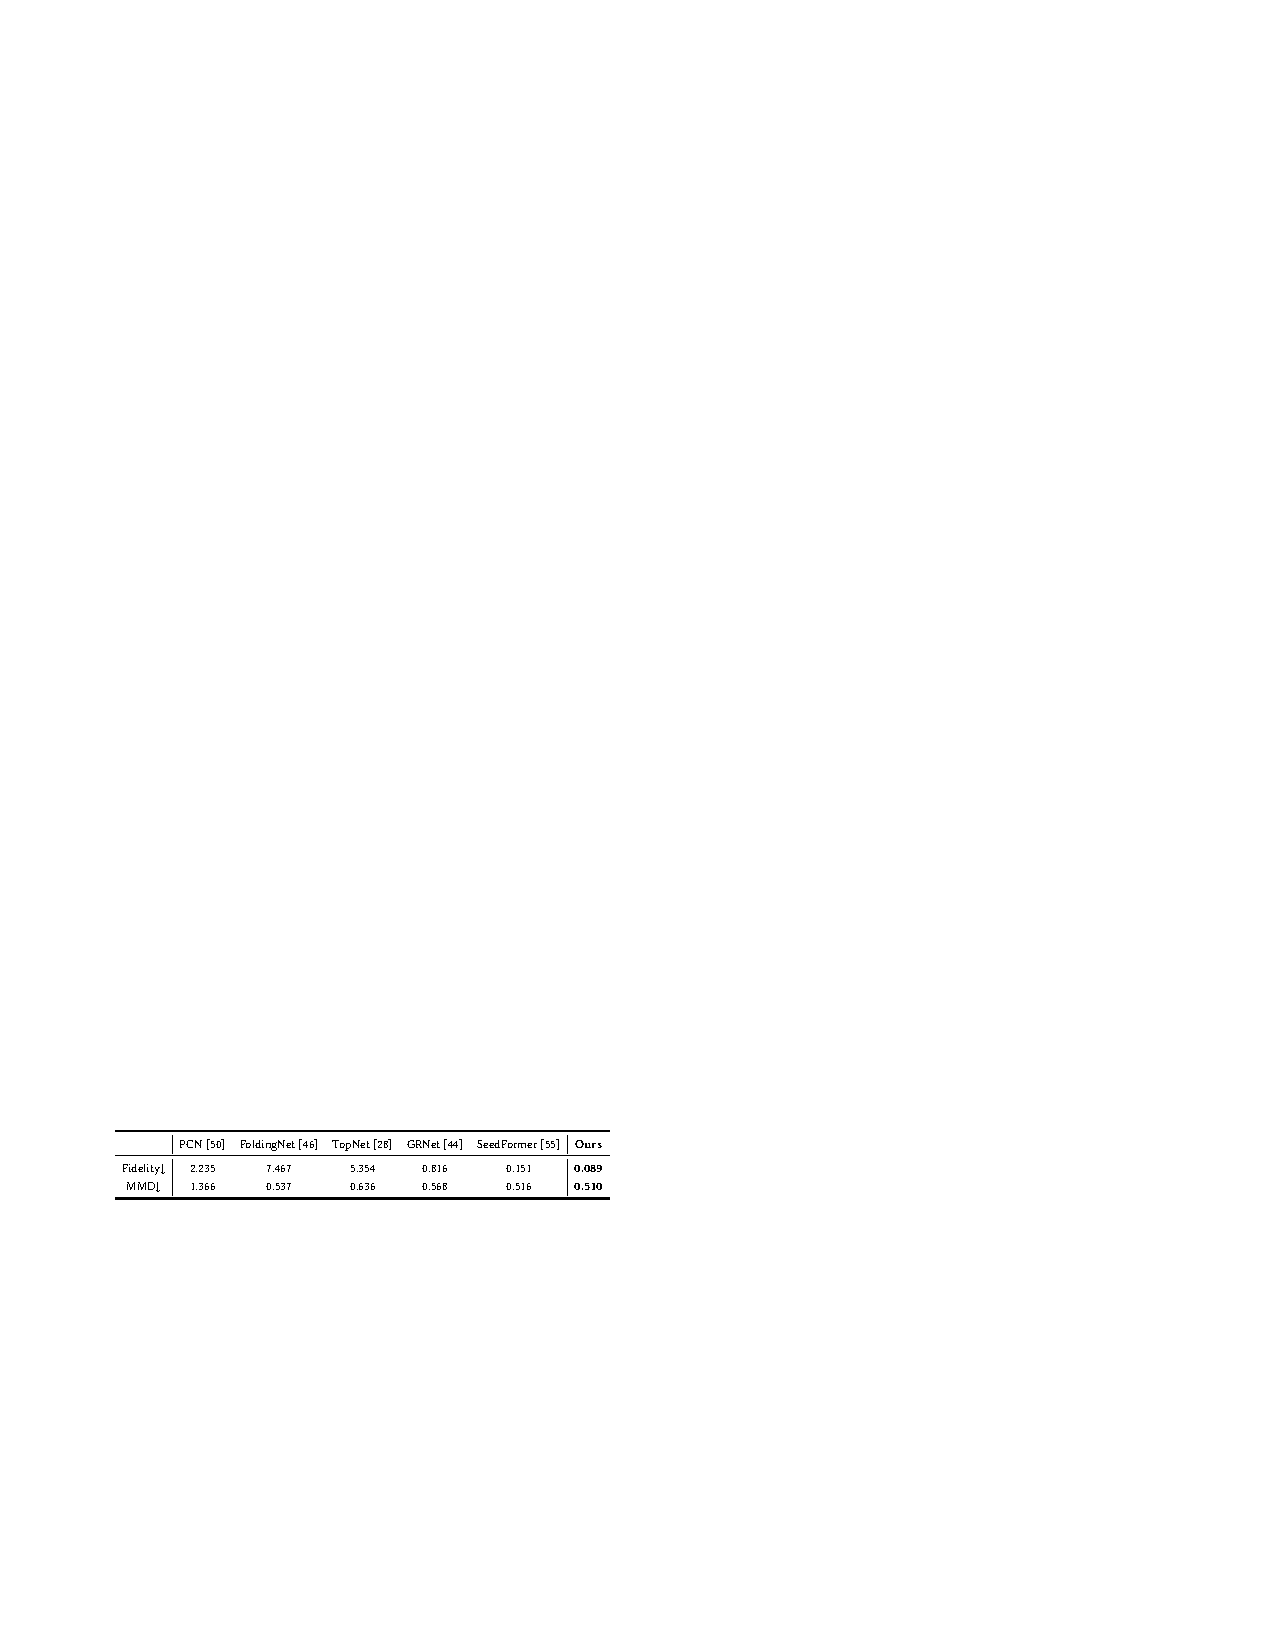
\includegraphics[width=\textwidth]{images/table-KITTI.pdf}
        \end{center}
        \vspace{-1.5em}
        %%%%%%%%%%%%%%%%%%%%%%%% figure  %%%%%%%%%%%%%%%%%%%%%%%%%%%%%
        \begin{center}
            % Qualitative comparison on KITTI benchmark \\[0.2em]
            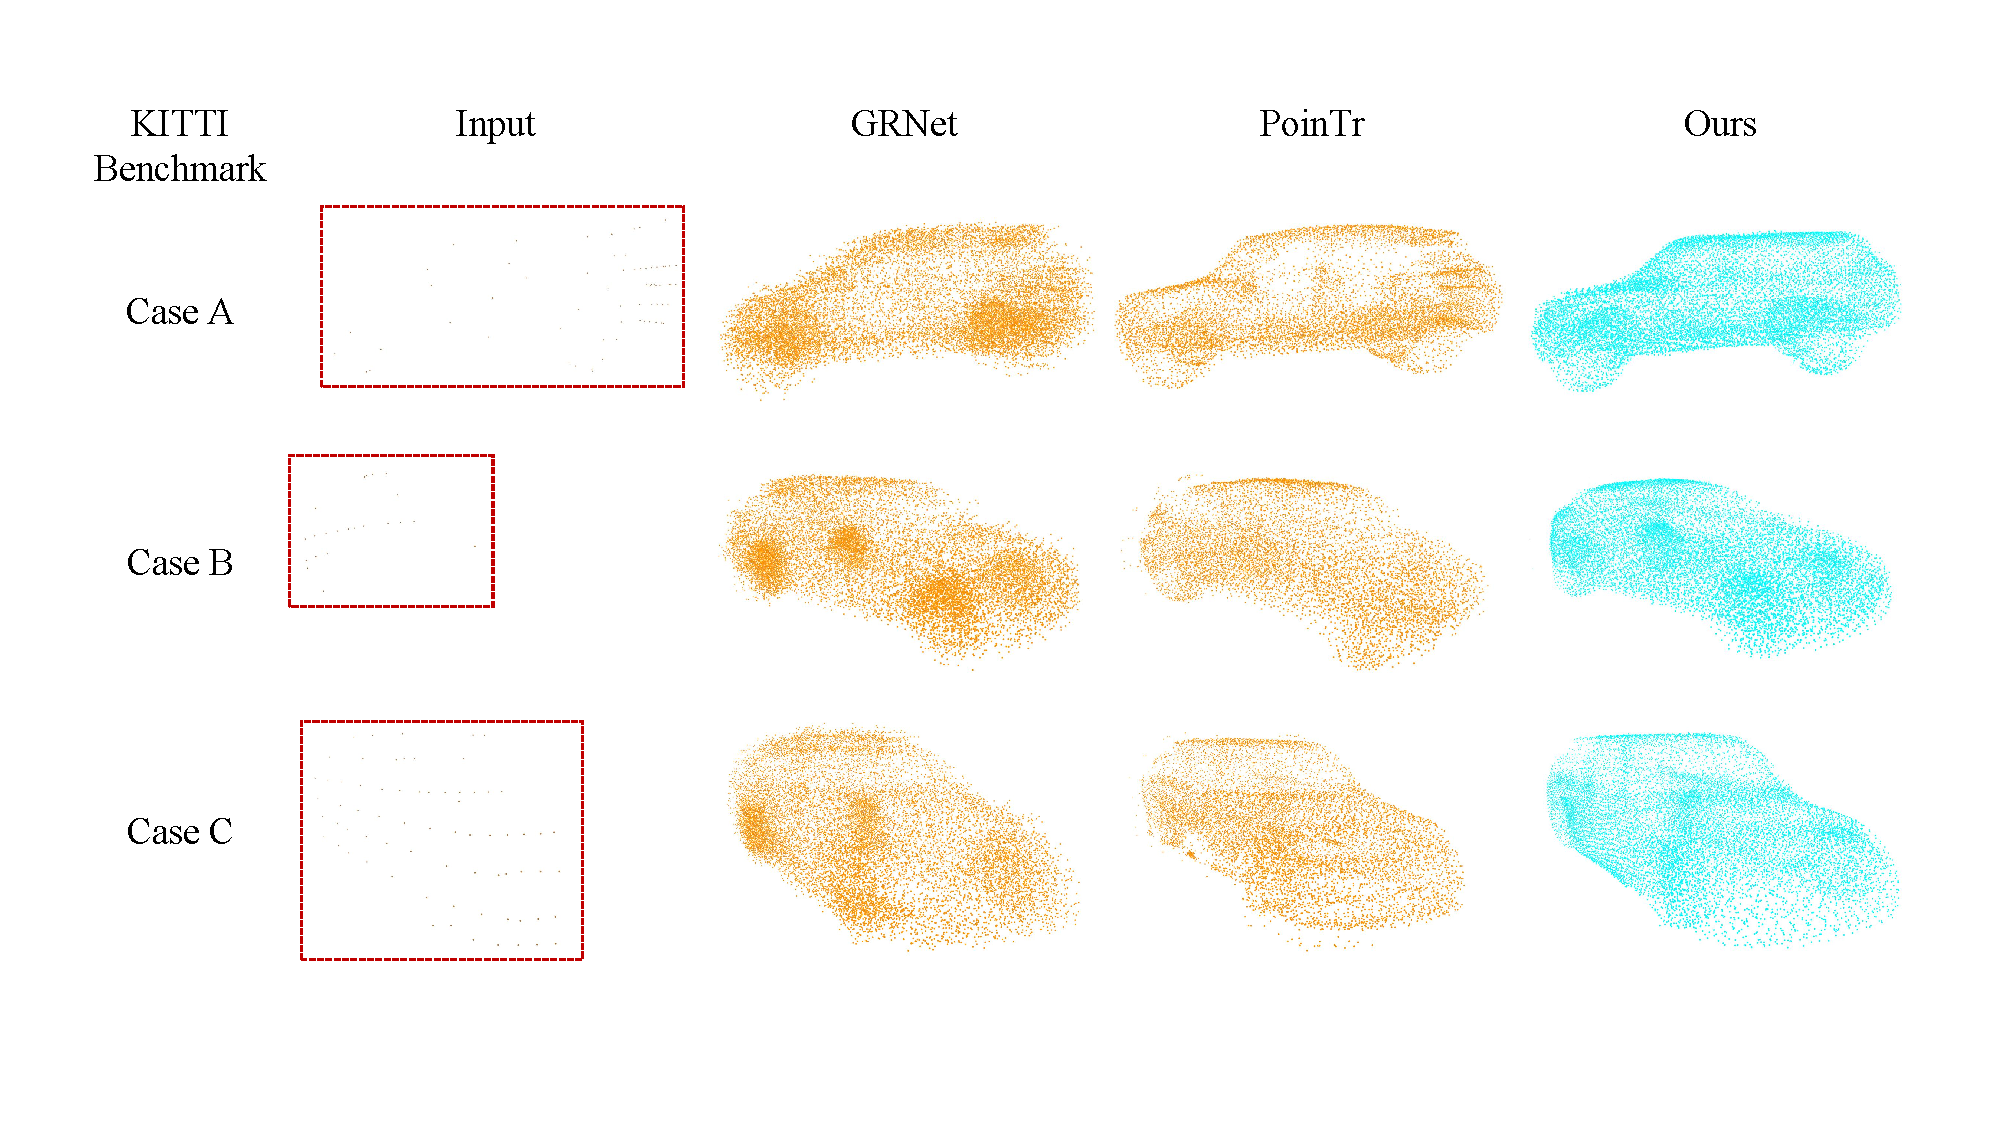
\includegraphics[width=\textwidth]{images/result-KITTI.pdf}
        \end{center}
        
    \end{minipage}\hfill
    %%%%%%%%%%%%%%%%%%%%%%%%%%%%%%%%%%%%%%%%%%%%%%%%%%%%%%%%%%%%%%%%%%
    %%%%%%%%%%%%%%%%% second column %%%%%%%%%%%%%%%%%%%%%%%%%%%%%%%%%%
    %%%%%%%%%%%%%%%%%%%%%%%%%%%%%%%%%%%%%%%%%%%%%%%%%%%%%%%%%%%%%%%%%%
    \begin{minipage}[t]{0.49\textwidth}
        %%%%%%%%%%%%%%%%%%%%%%%% ShapeNet-55/34  %%%%%%%%%%%%%%%%%%%%%%%%%%%%%
        \vspace{-0.5em}
        \textbf{\color{ctitle}Comparison on ShapeNet-55/34 Benchmark:}
        %%%%%%%%%%%%%%%%%%%%%%%% table  %%%%%%%%%%%%%%%%%%%%%%%%%%%%%
        \vspace{-0.6em}
        \begin{center}
            Quantitative results on ShapeNet-55 benchmark \\
            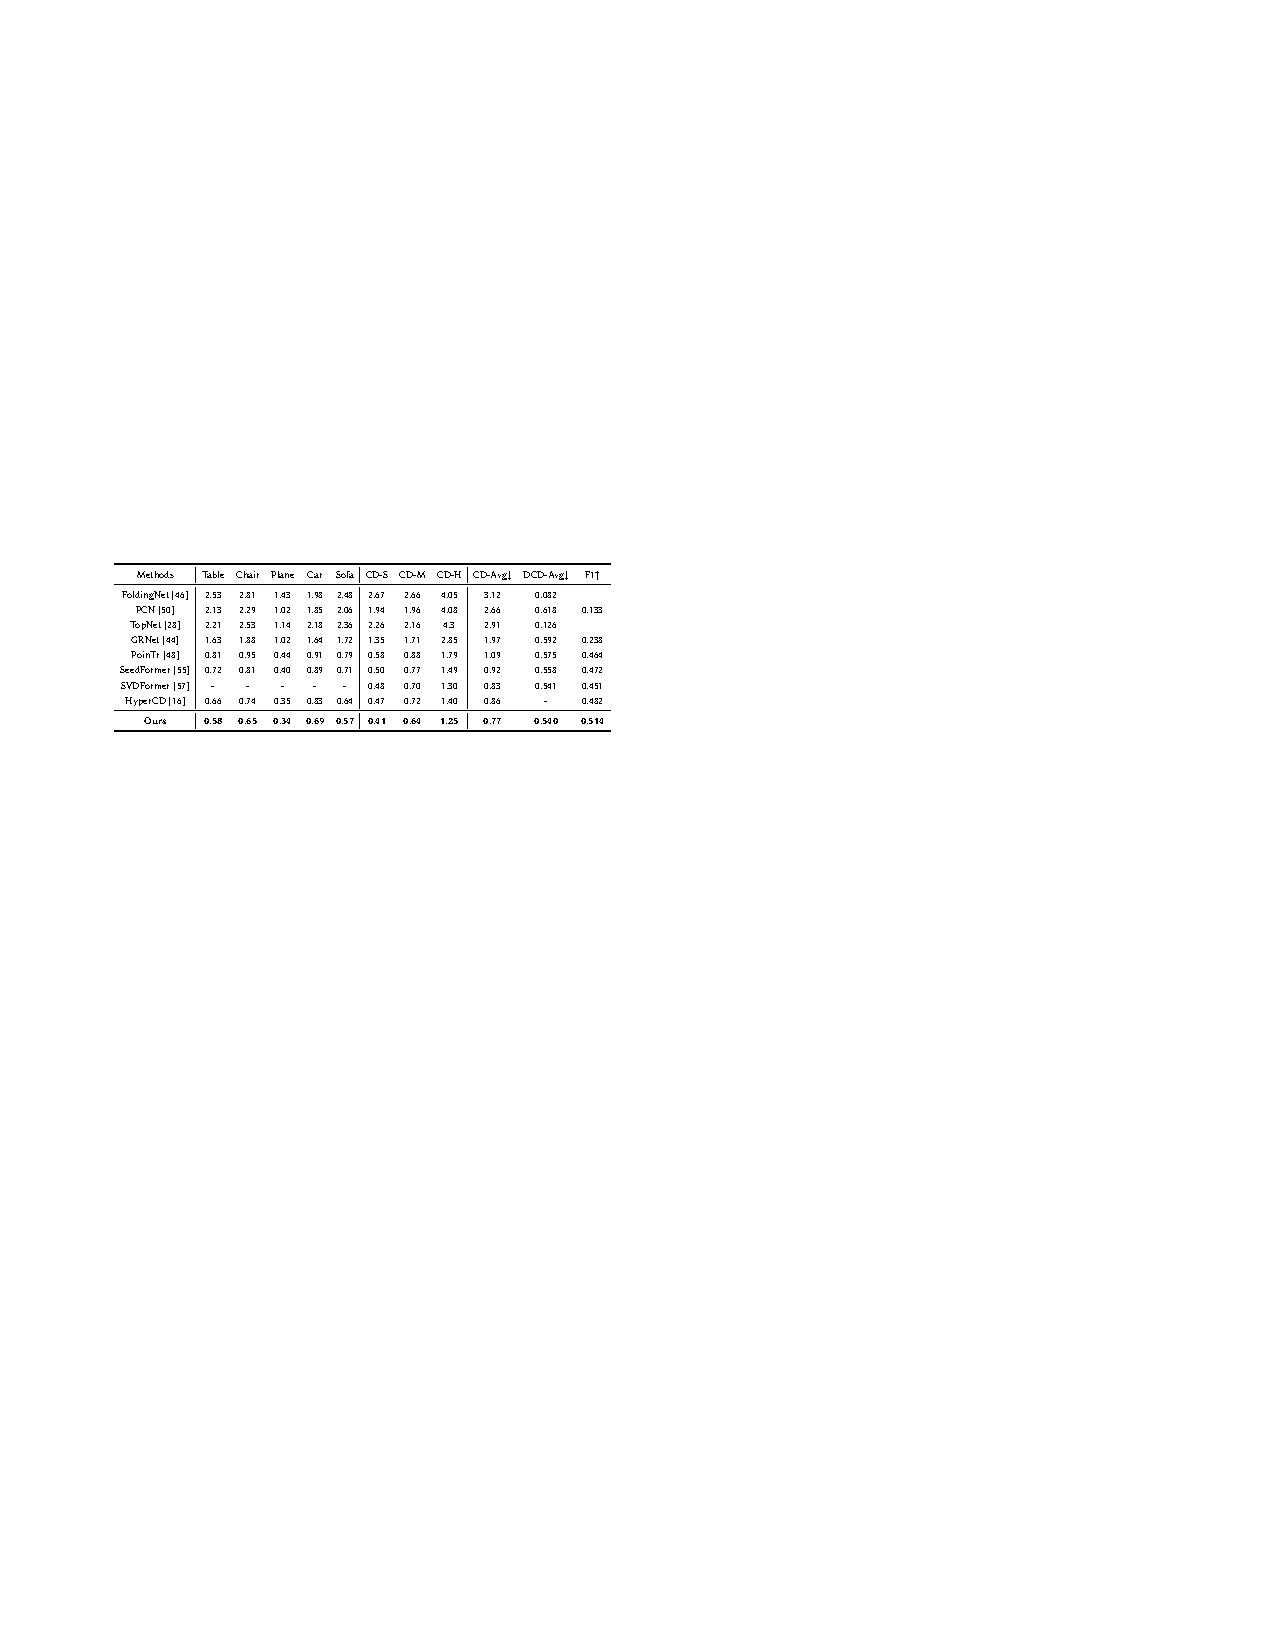
\includegraphics[width=\textwidth]{images/table-SP55.pdf}
        \end{center}
        \vspace{-1.8em}
        \begin{center}
            Quantitative results on ShapeNet-34/21 benchmark \\
            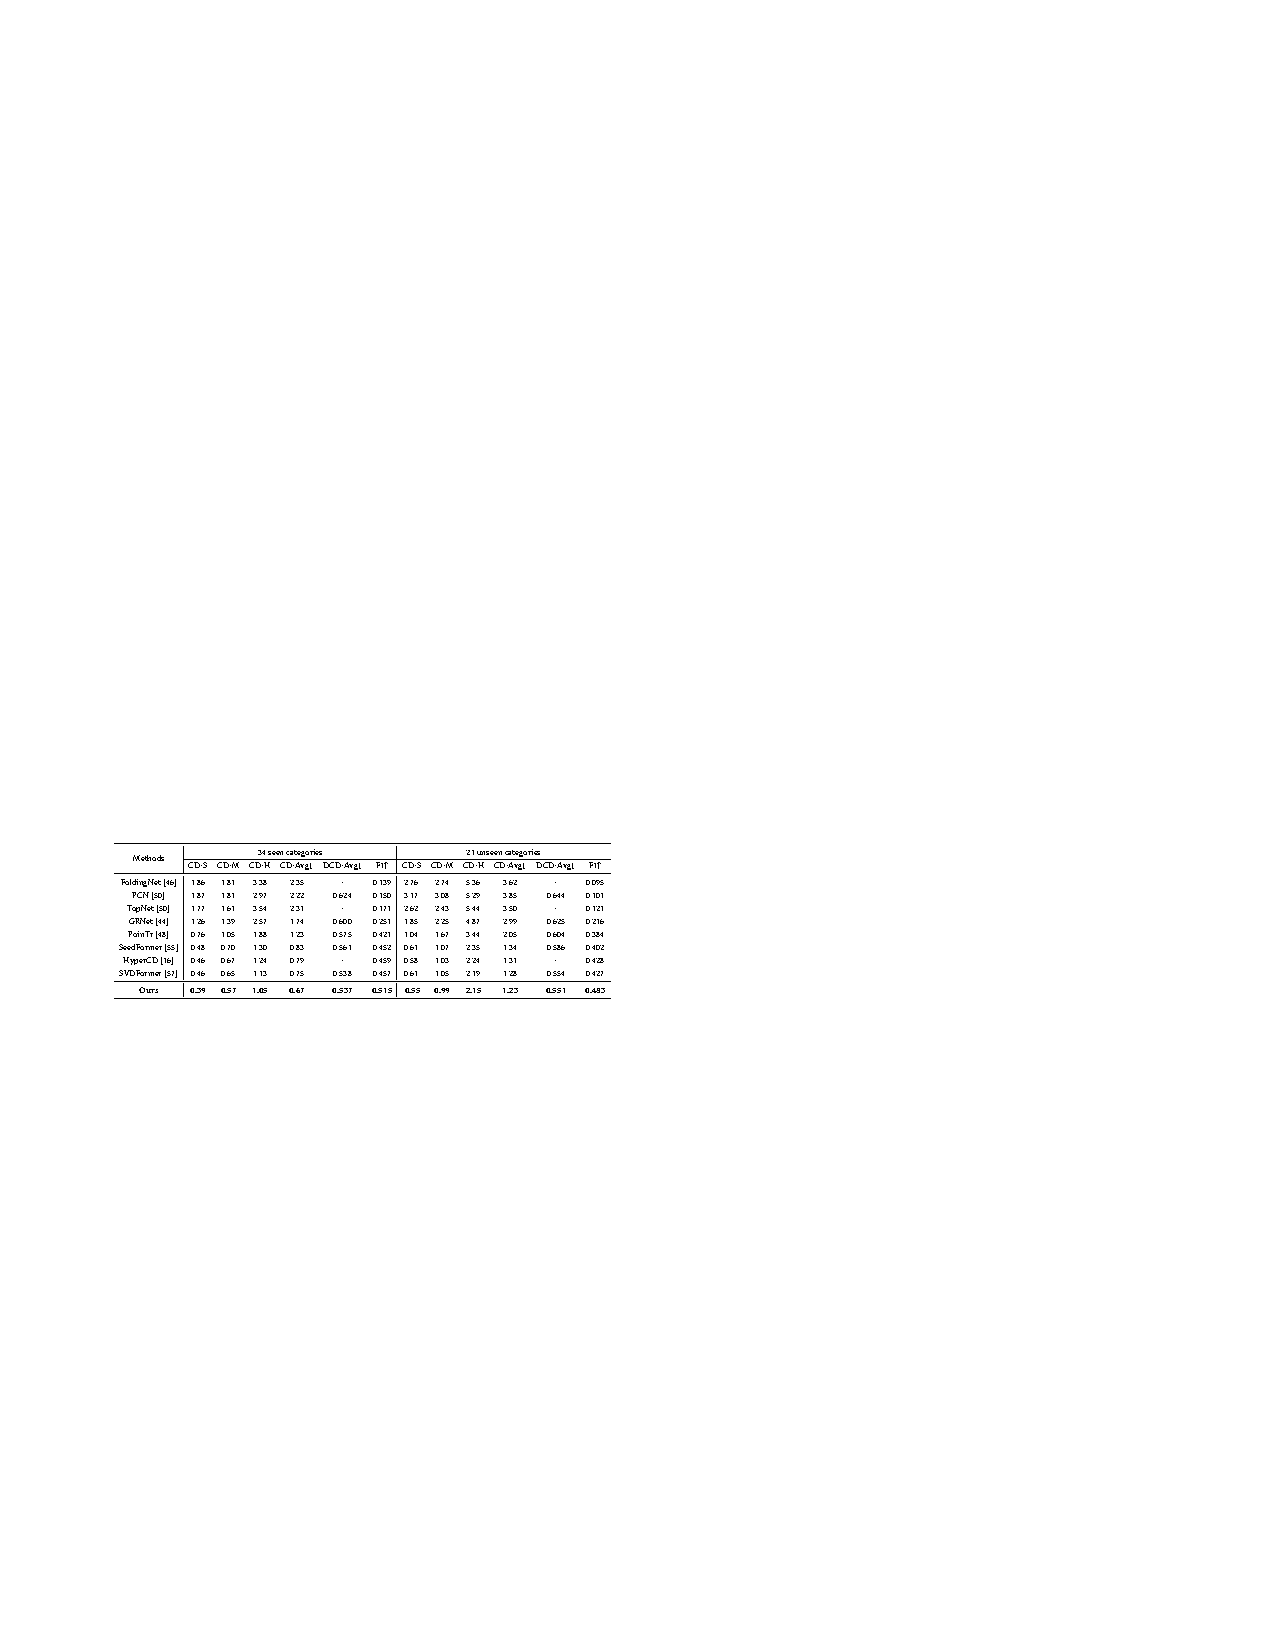
\includegraphics[width=\textwidth]{images/table-SP34.pdf}
        \end{center}
        \vspace{-1.8em}
        %%%%%%%%%%%%%%%%%%%%%%%% figure  %%%%%%%%%%%%%%%%%%%%%%%%%%%%%
        \begin{center}
            Qualitative comparison on ShapeNet-55 benchmark \\[0.2em]
            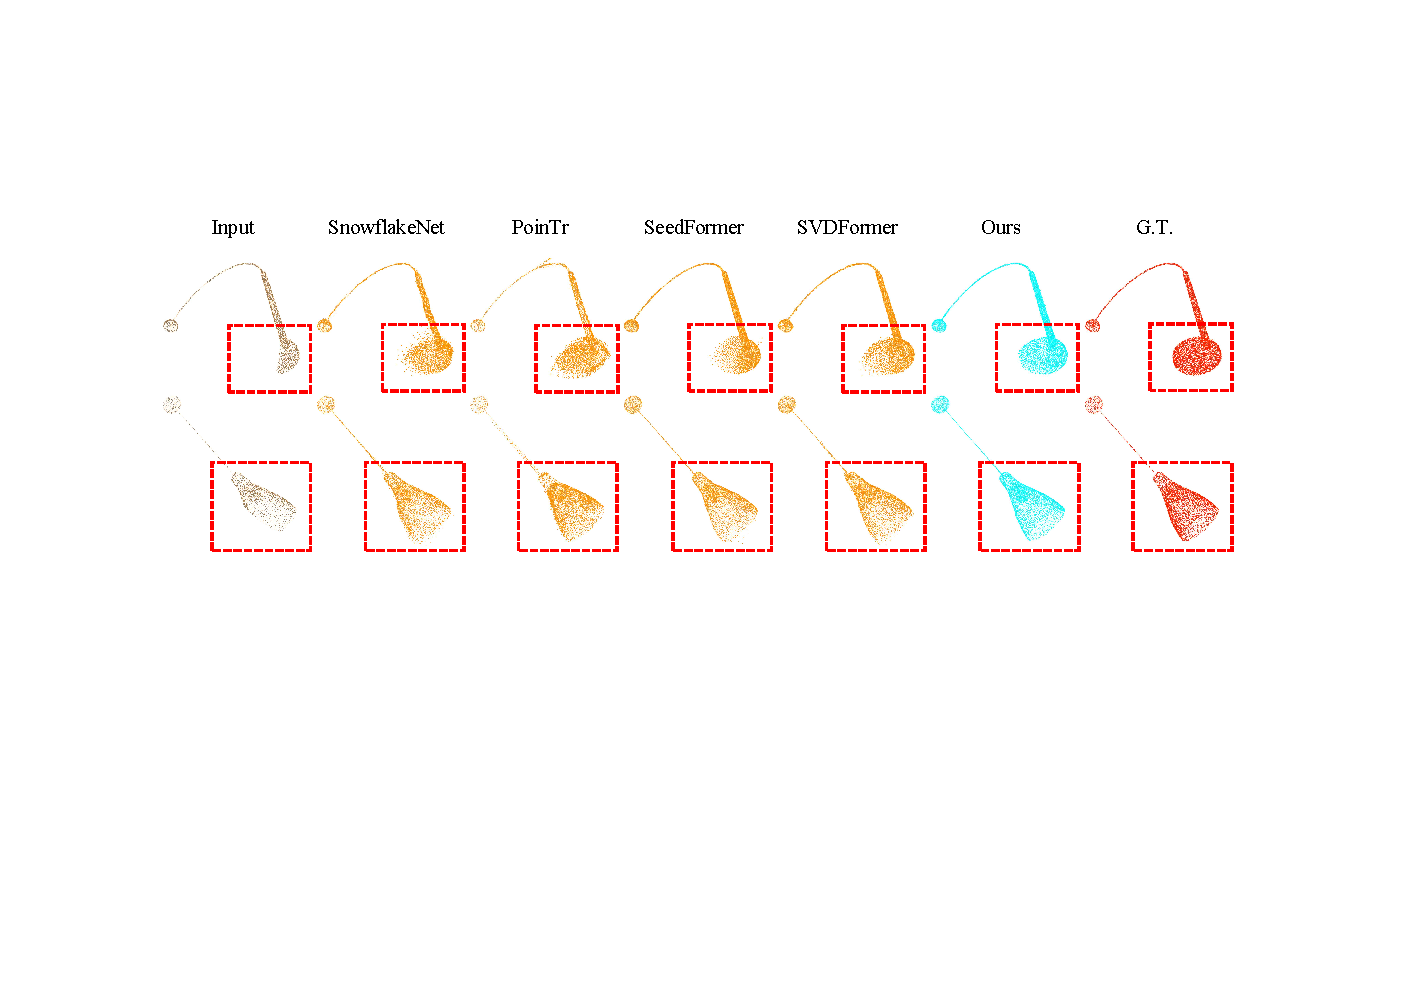
\includegraphics[width=\textwidth]{images/result-shapenet55.pdf}
        \end{center}
        \vspace{-1.3em}

        %%%%%%%%%%%%%%%%%%%%%%%% Ablation  %%%%%%%%%%%%%%%%%%%%%%%%%%%%%
        \textbf{\color{ctitle}Effectiveness of Improved Design Components:} \\
        %%%%%%%%%%%%%%%%%%%%%%%% table  %%%%%%%%%%%%%%%%%%%%%%%%%%%%%
        \begin{minipage}[t]{0.48\textwidth}
            \text{}
            \vspace{-1.5em}
            \begin{center}
                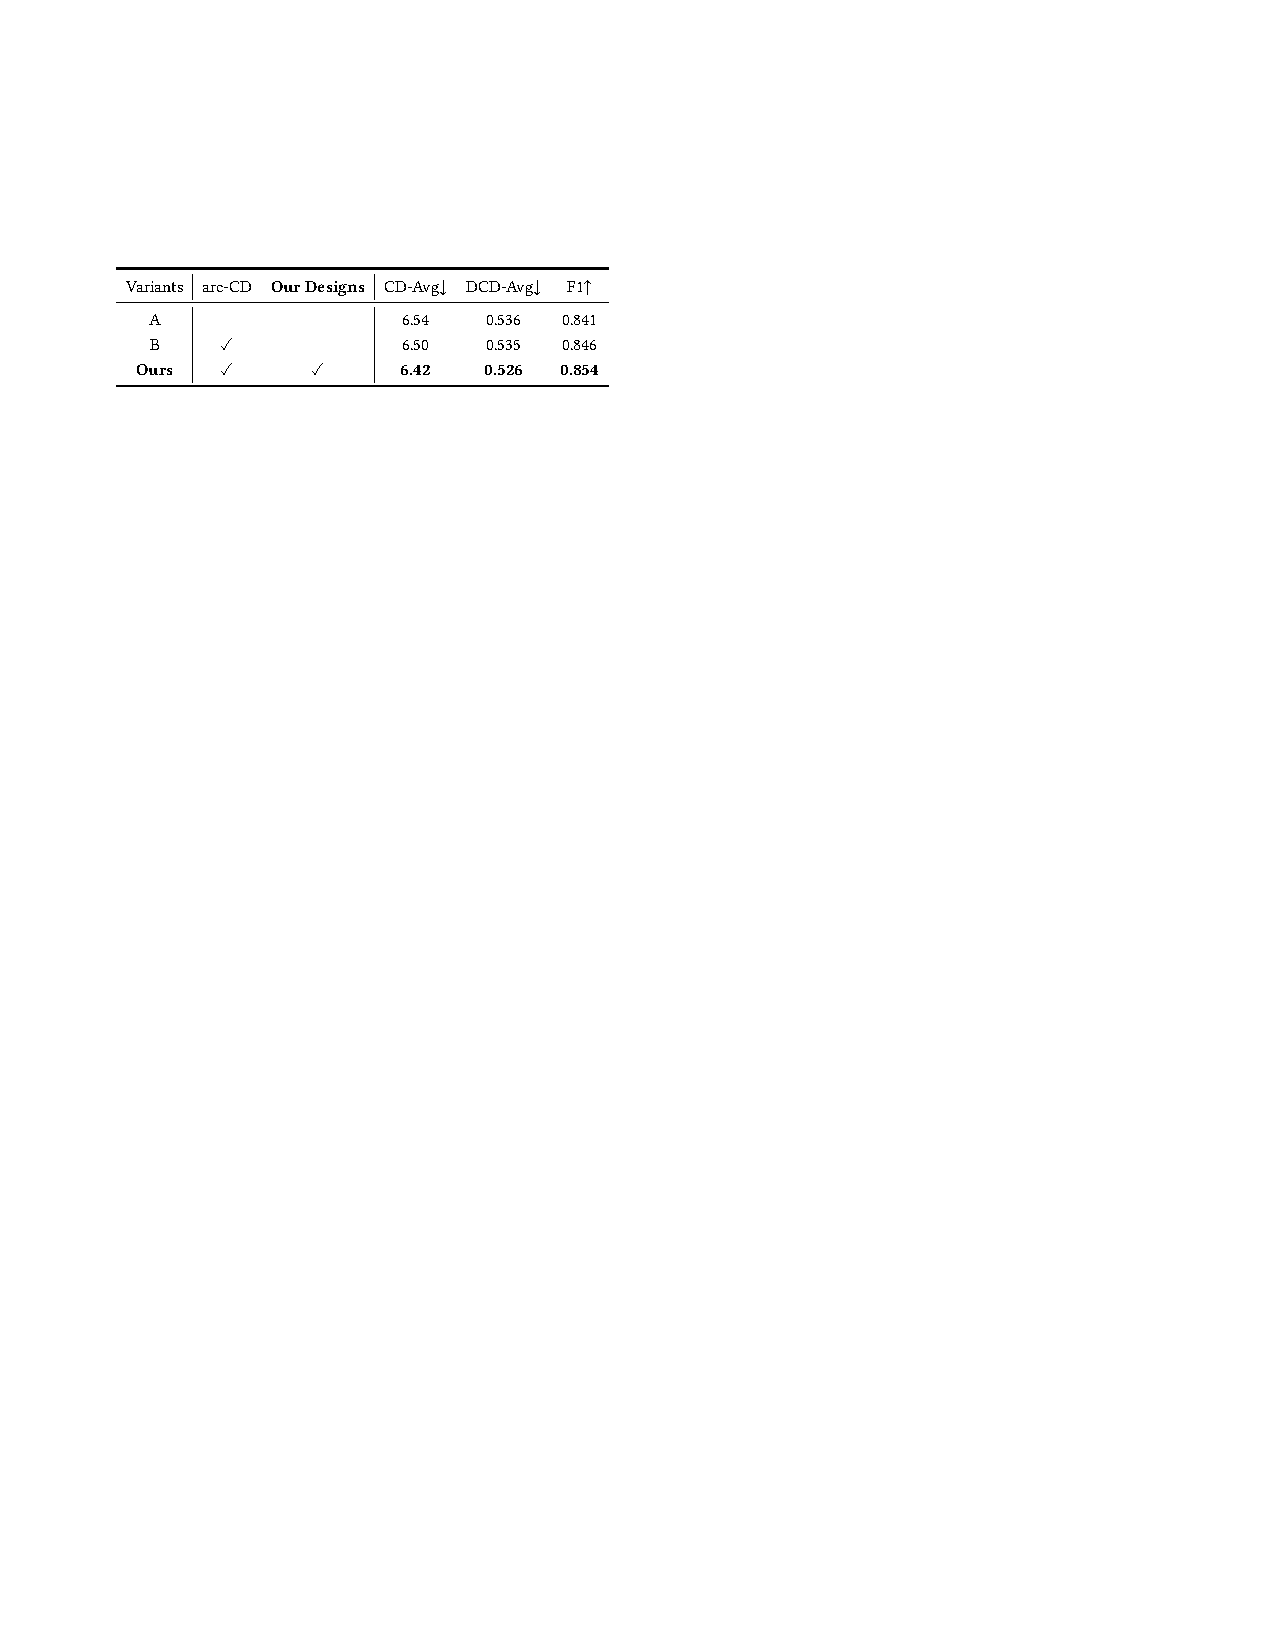
\includegraphics[width=\textwidth]{images/table-ablation-loss.pdf} \\
                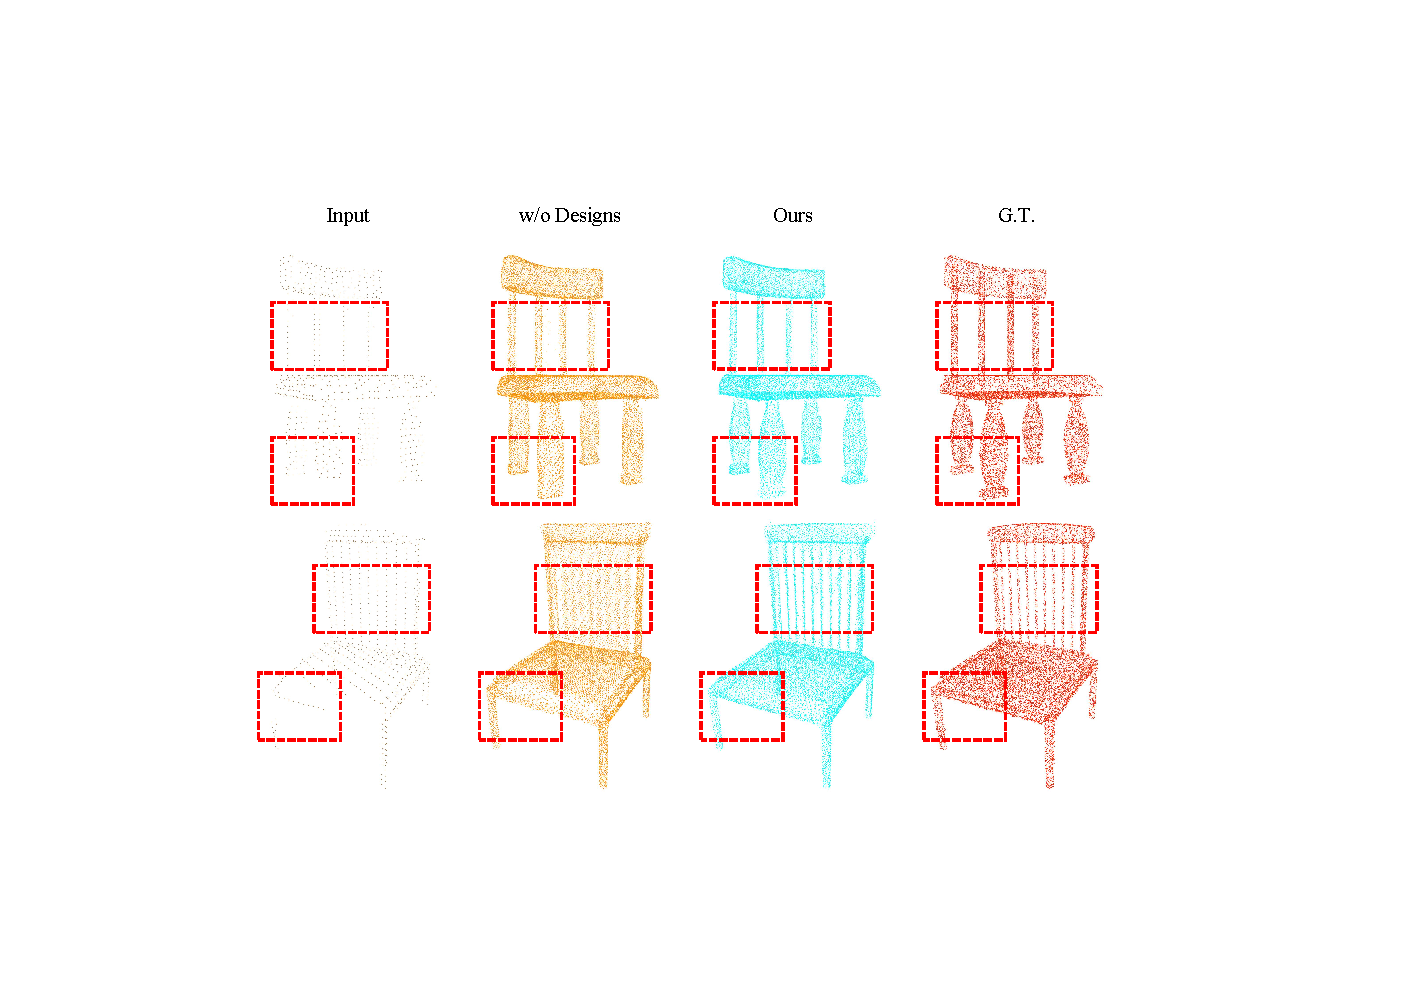
\includegraphics[width=\textwidth]{images/result-ablation-loss.pdf} \\
                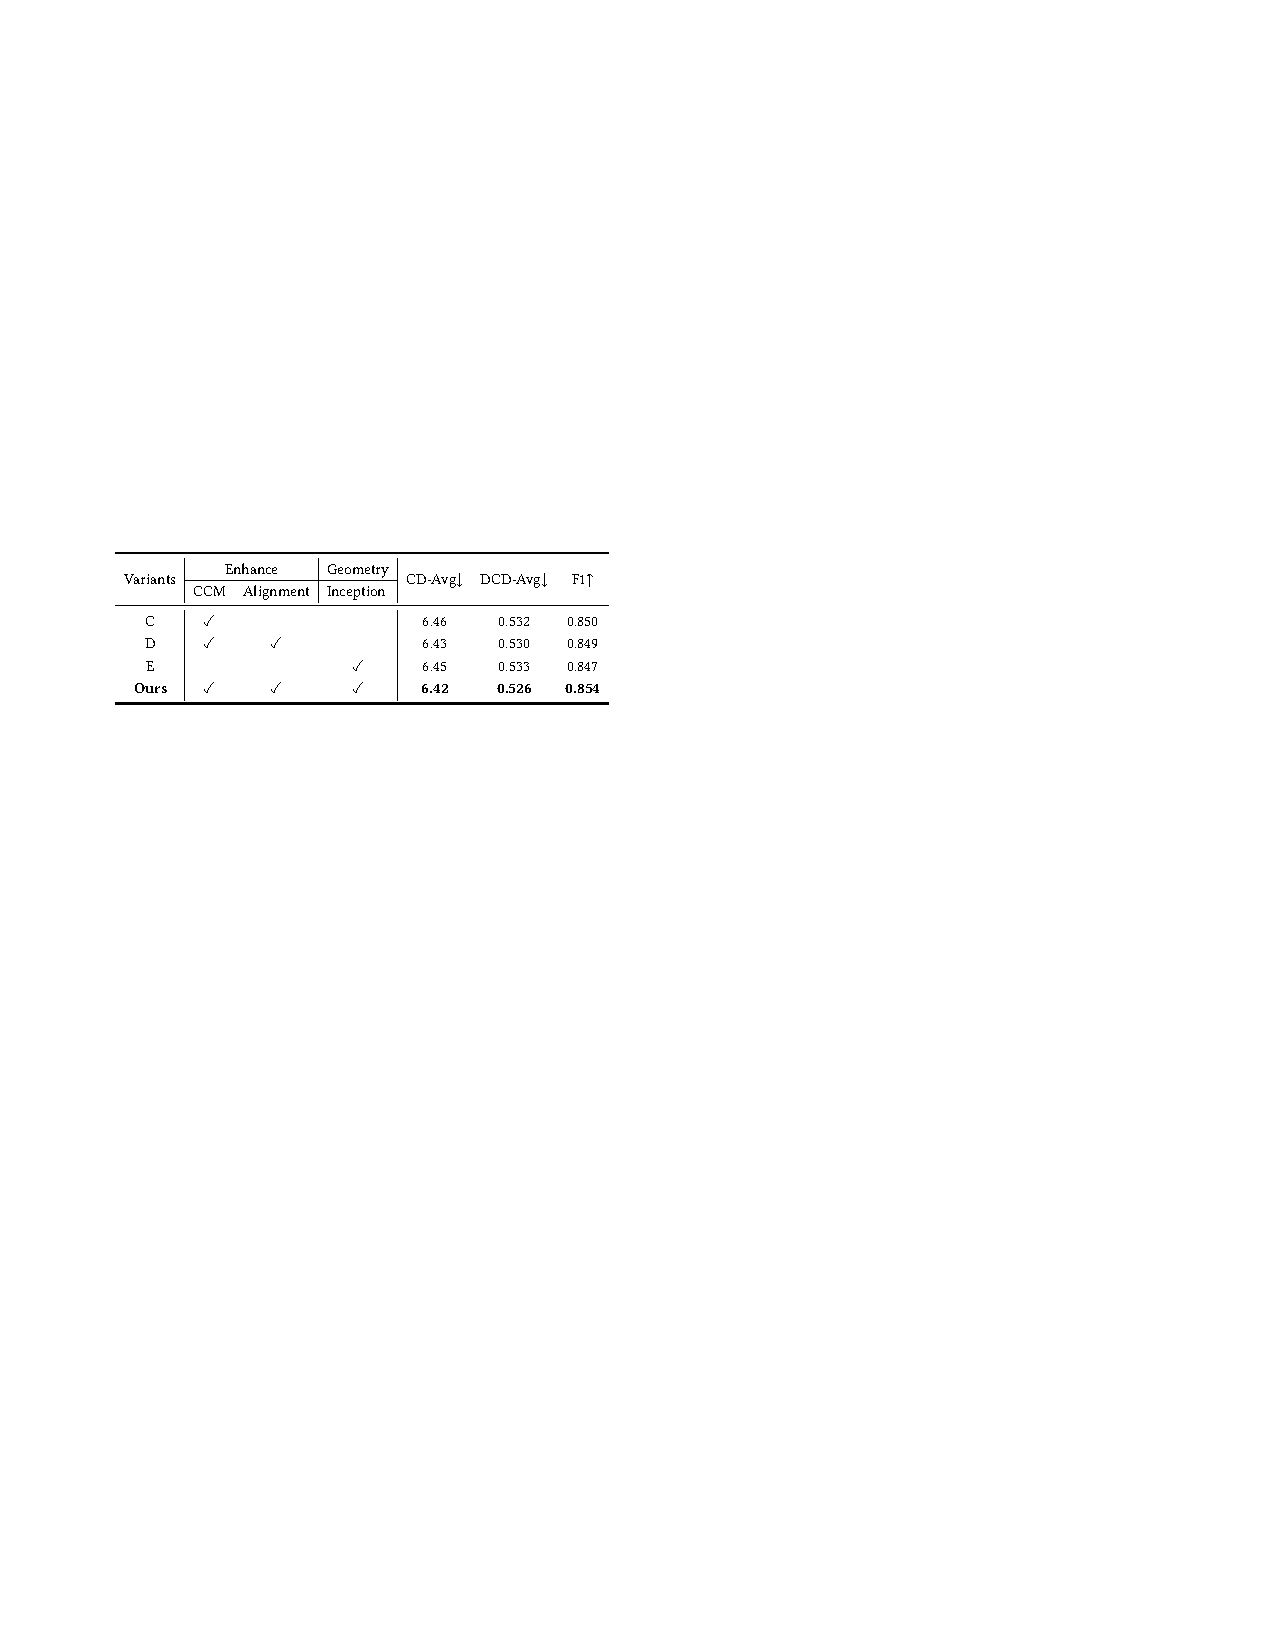
\includegraphics[width=\textwidth]{images/table-ablation-design.pdf}
            \end{center}
        \end{minipage}\hfill
        \begin{minipage}[t]{0.52\textwidth}
            \text{}
            \vspace{-1.5em}
            \begin{center}
                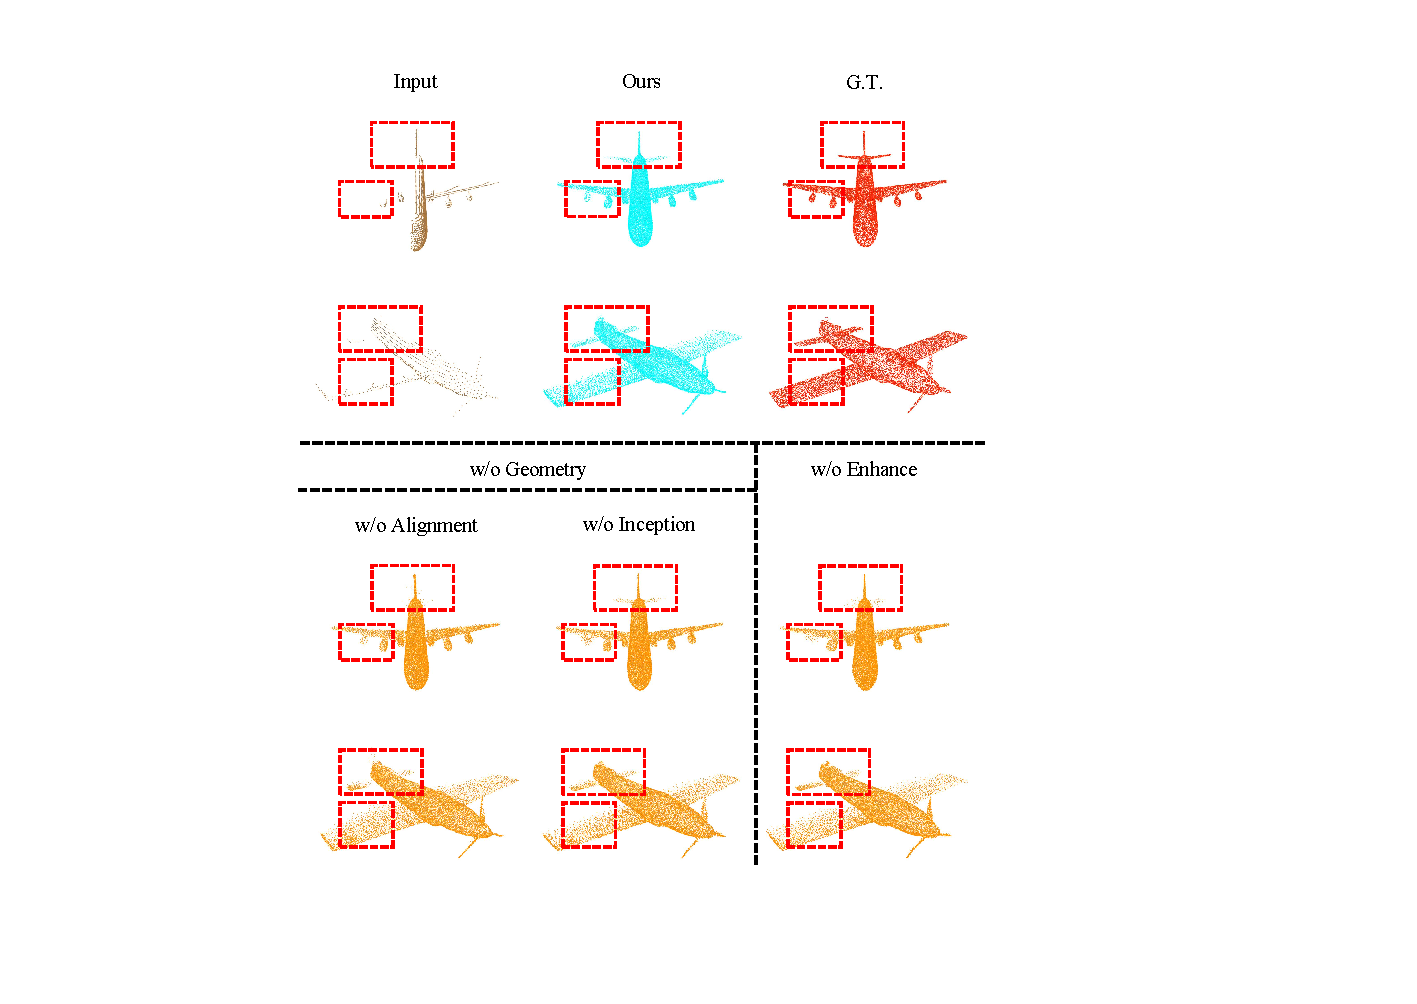
\includegraphics[width=\textwidth]{images/result-ablation-design.pdf}
            \end{center}
        \end{minipage}
    \end{minipage}

}
\end{poster}
\end{document}